\documentclass{article}

\usepackage[margin=1in]{geometry}
\usepackage{graphicx}
\usepackage{amsmath}
\usepackage{amsfonts}
\usepackage{float}

\author{Zachary Vogel}
\date{\today}
\title{Notes in ECEN 5448}

\begin{document}
\maketitle


\section*{What do we want}

\begin{itemize}
    \item analyze modes to determine rise time, \textbf{settle time}
    \item Analyze how sampling frequency effects performance
    \item figure out feedword control.
    \item $F_{CL}$ inverse of closed loop. Can be acausal because you know input.
    \item this is genrally for reference tracking.
    \item assume there aren't any dynamics between teh measured and actuation.
    \item can use matlabs tools, but analyze why matlabs tools work.
    \item Then figure out how much better we can do with feedforward.
\end{itemize}

\begin{figure}[H]
    \centering
    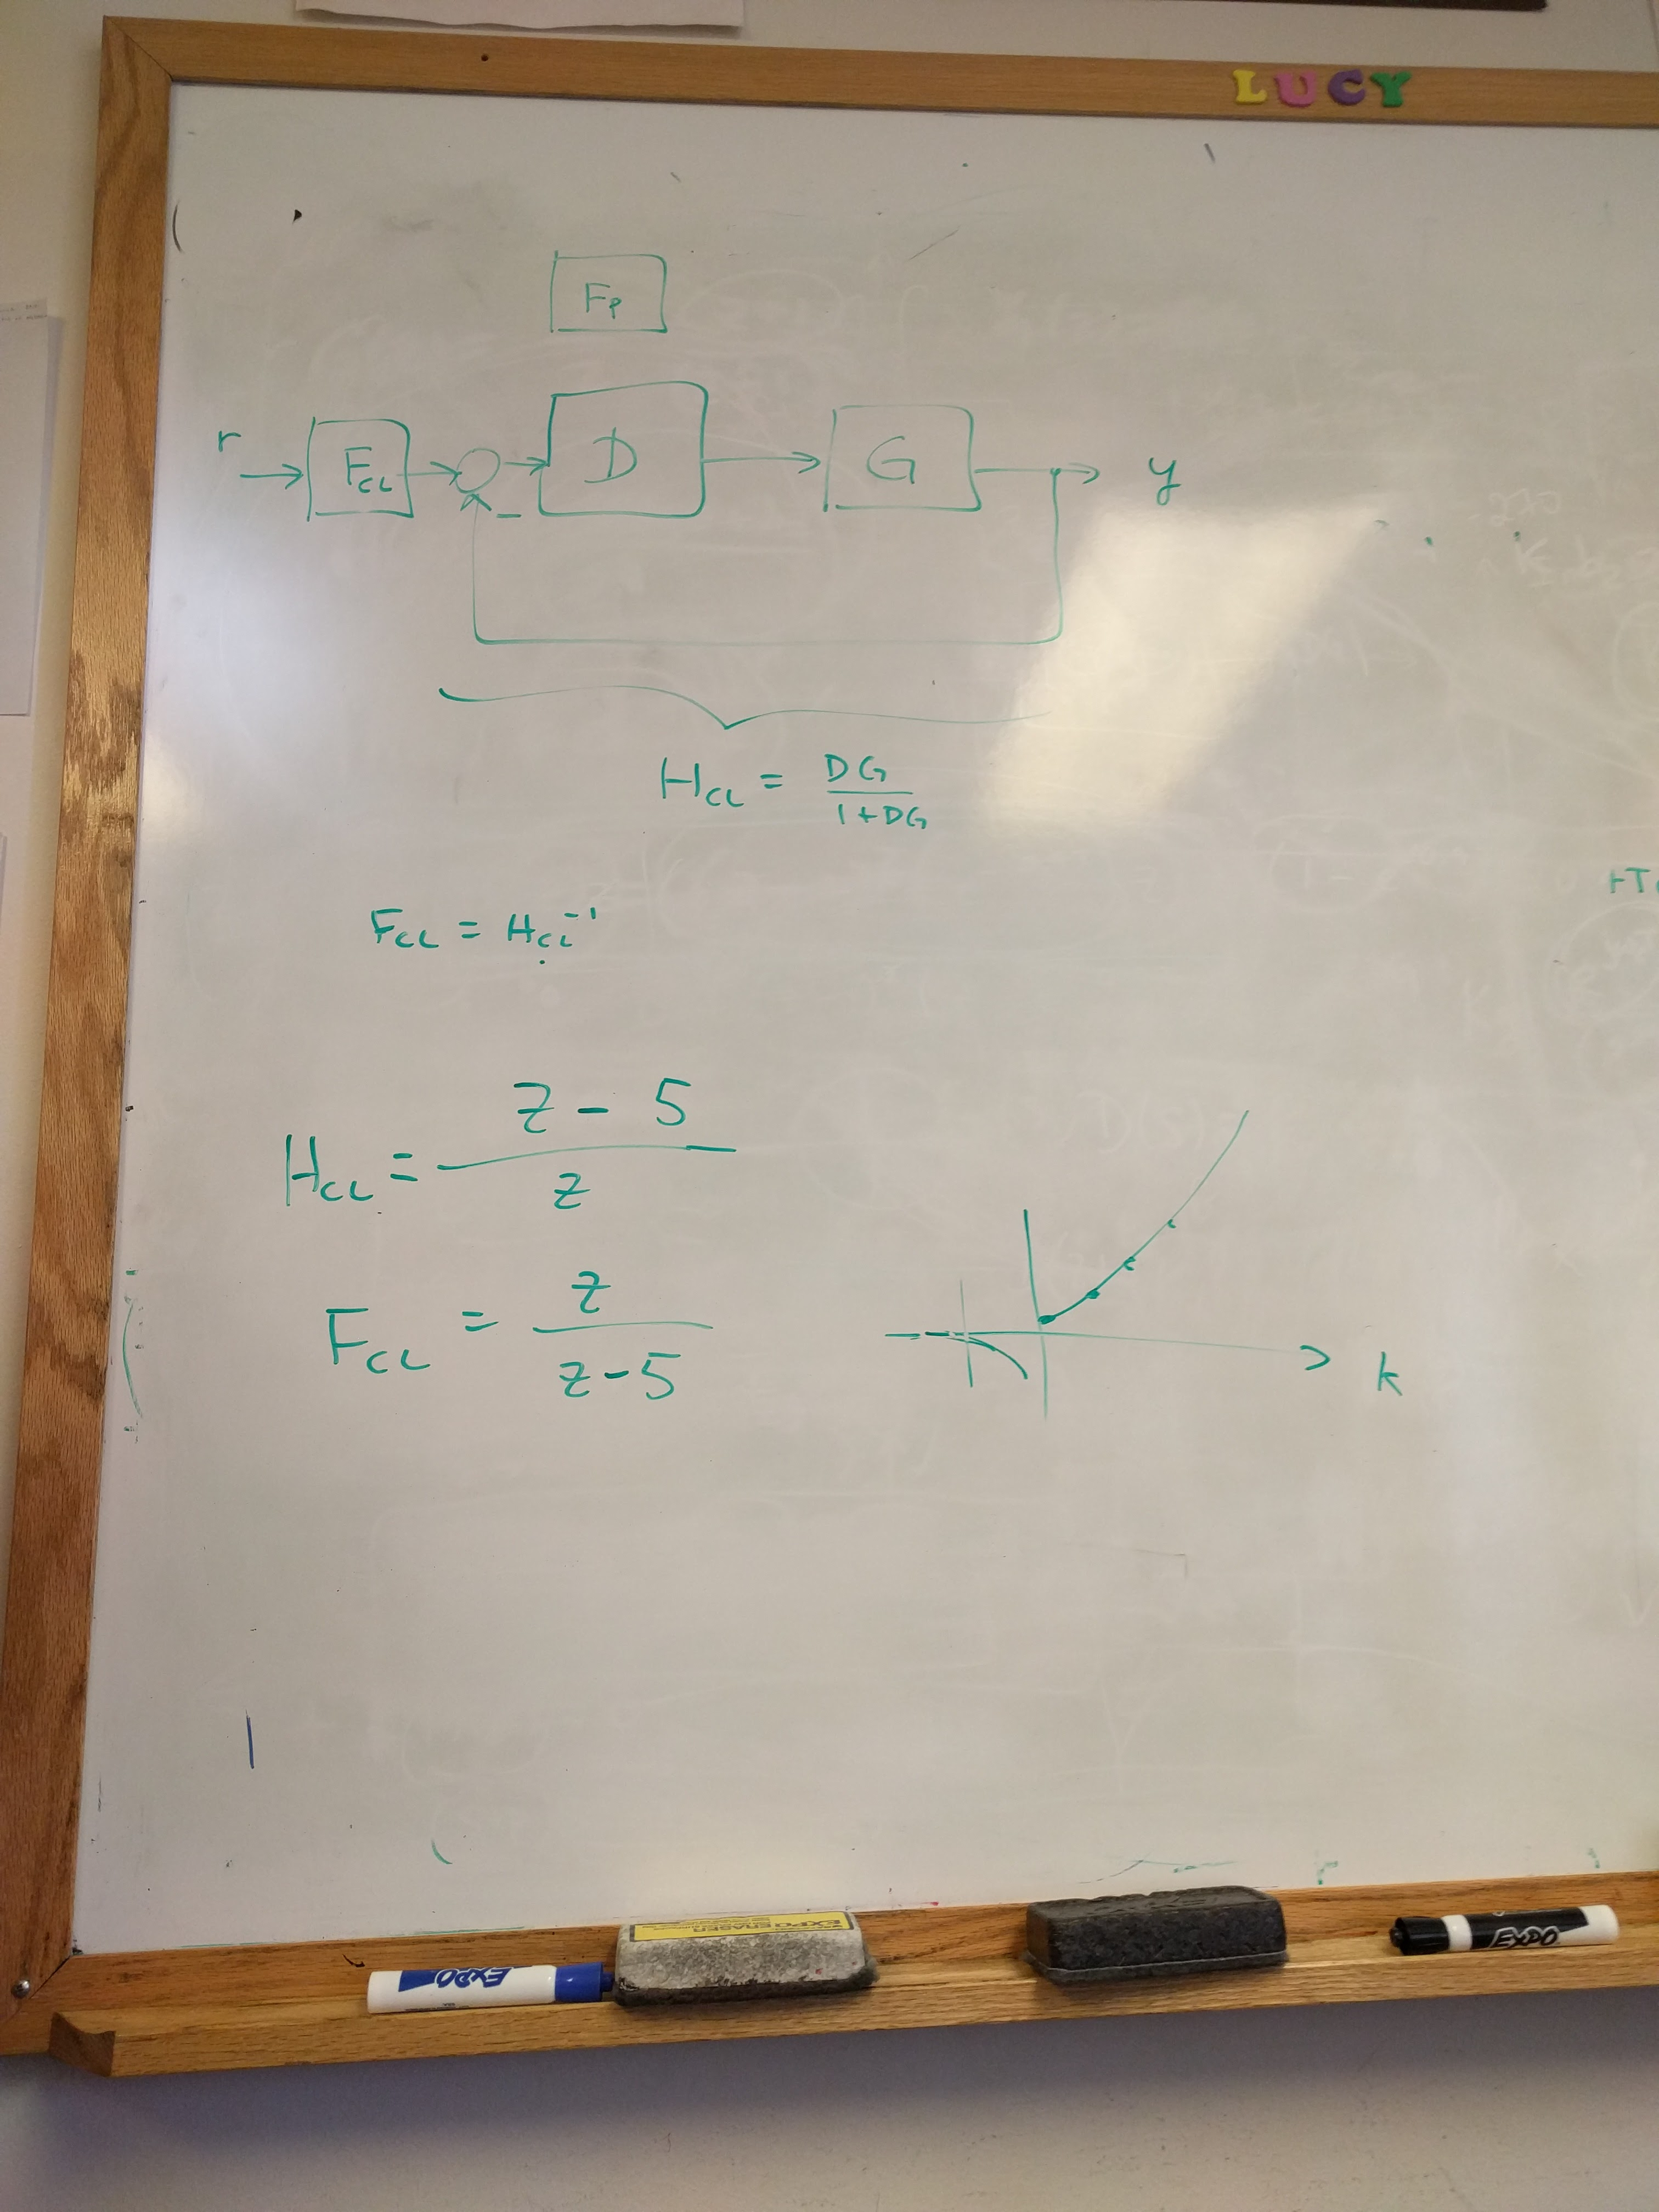
\includegraphics[width=0.8\textwidth]{pic1.jpg}
\end{figure}

\begin{figure}[H]
    \centering
    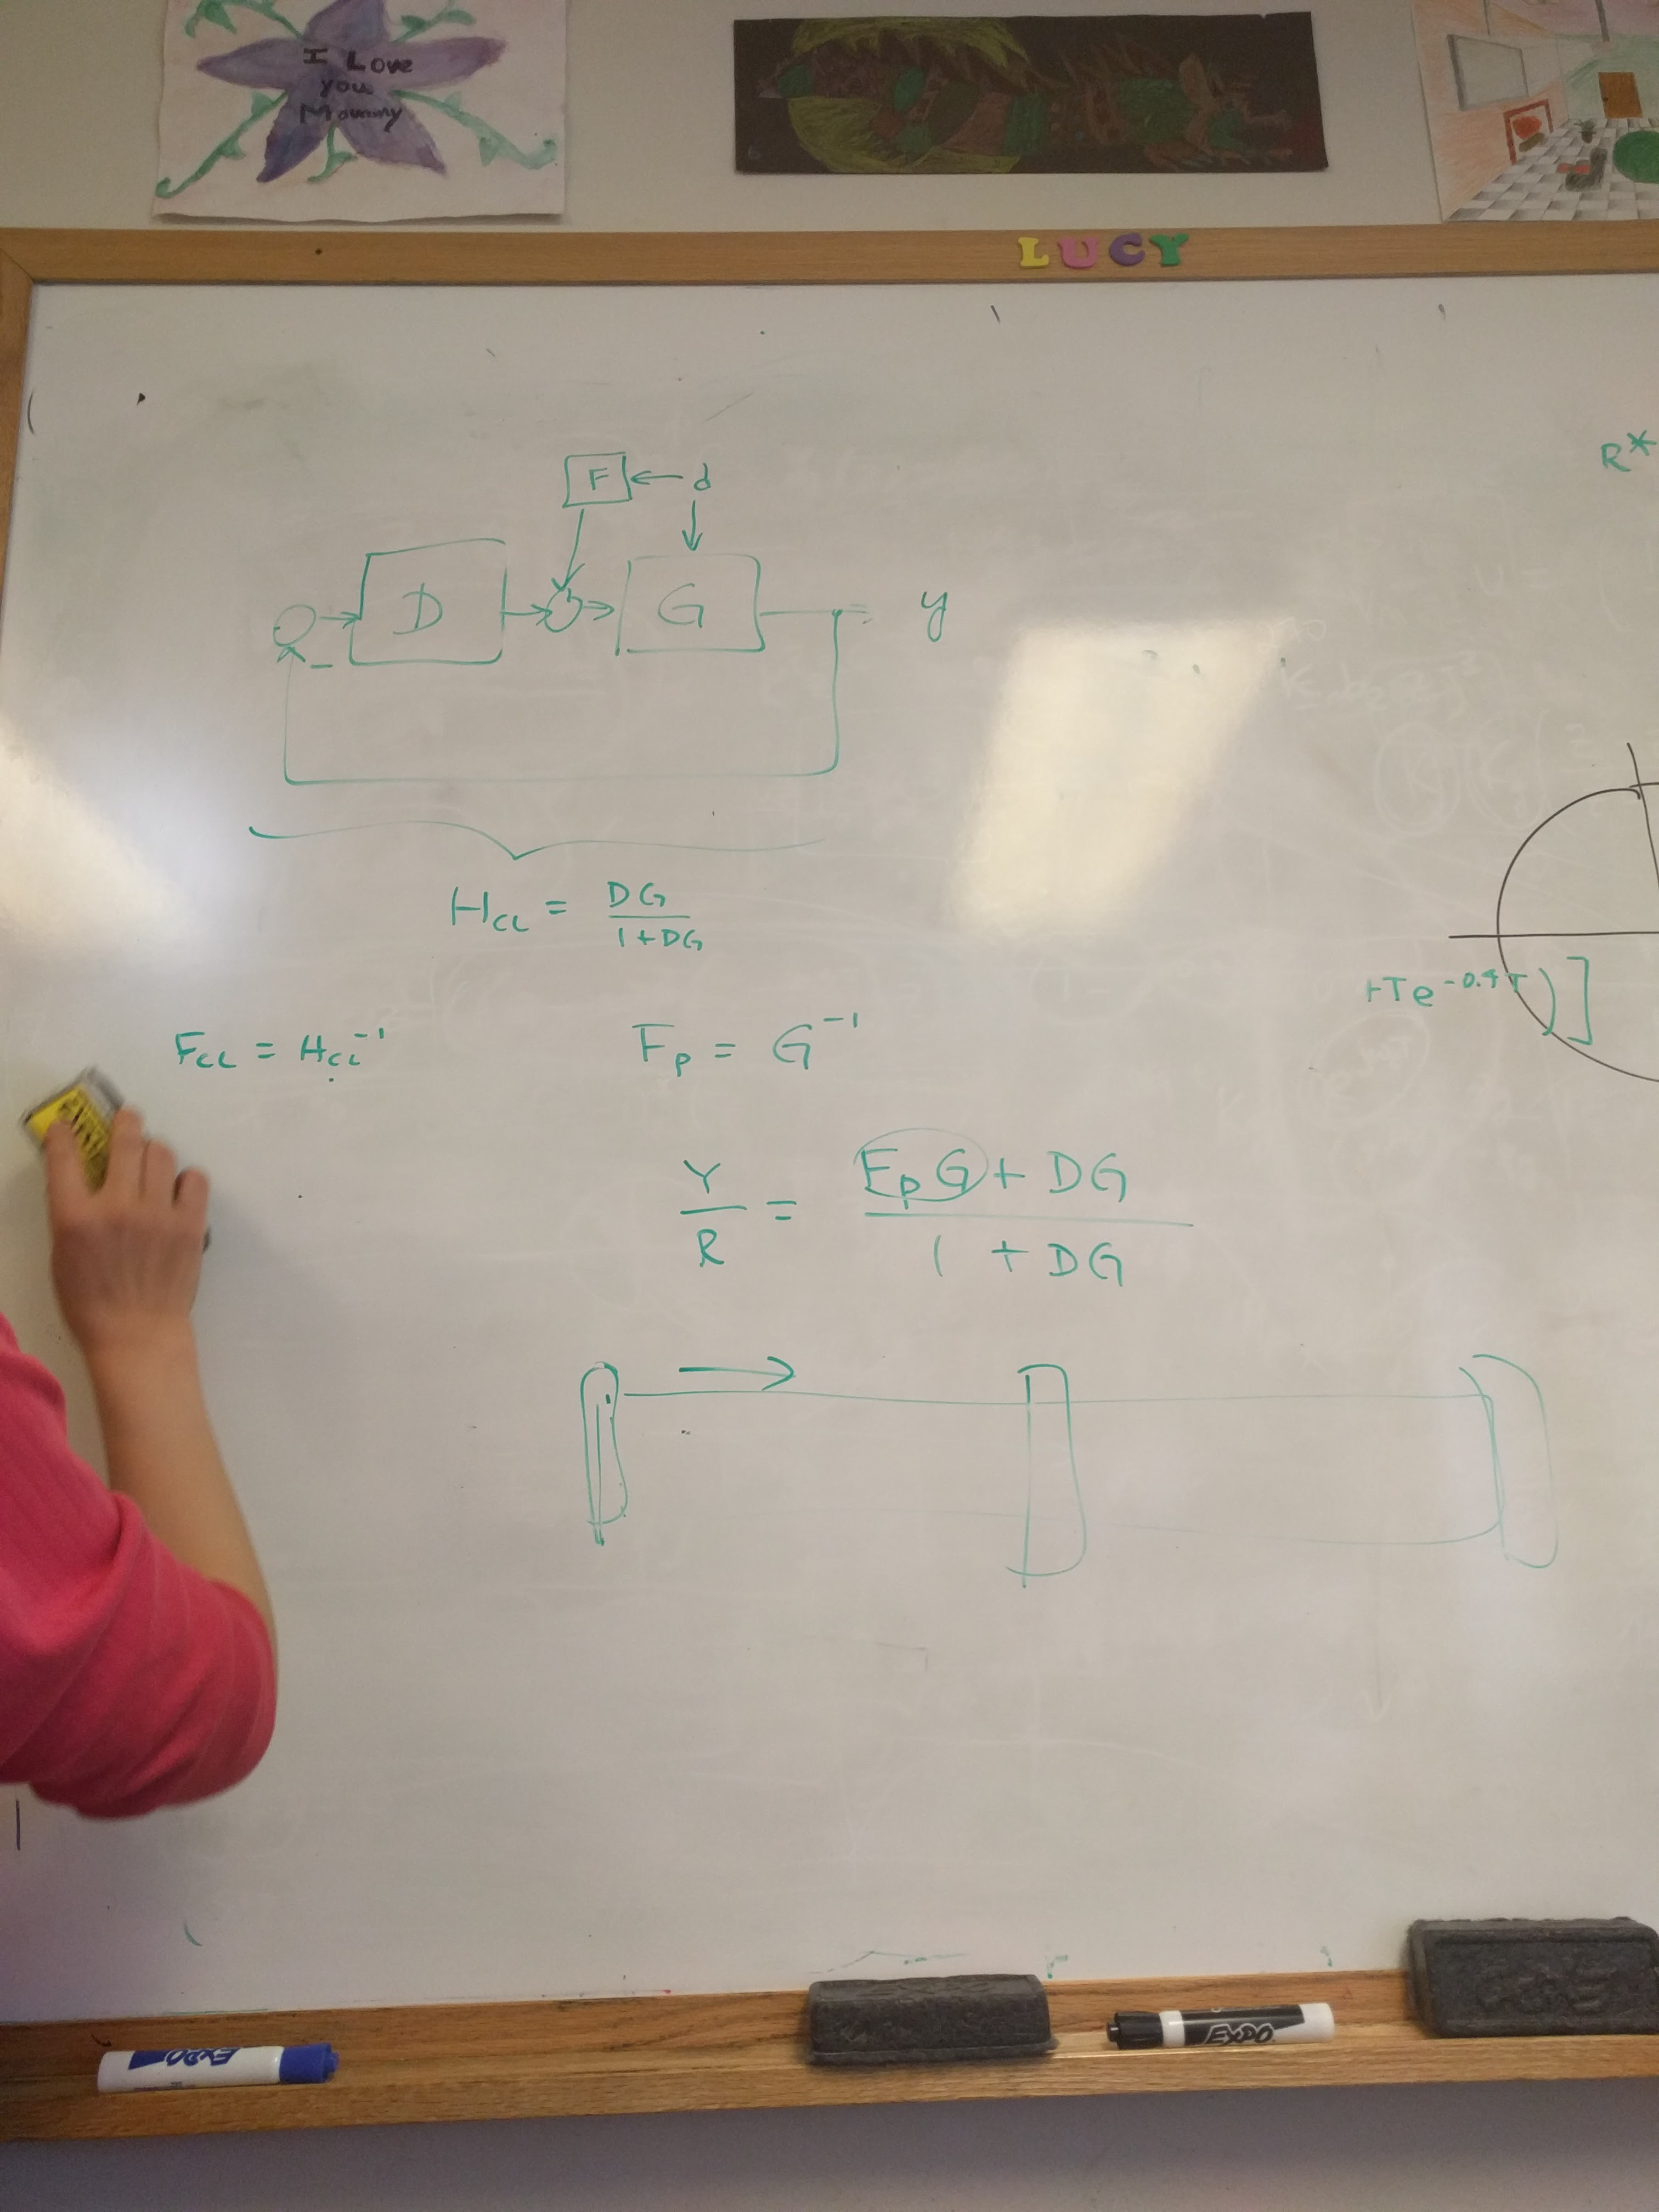
\includegraphics[width=0.8\textwidth]{pic2.jpg}
\end{figure}

\begin{figure}[H]
    \centering
    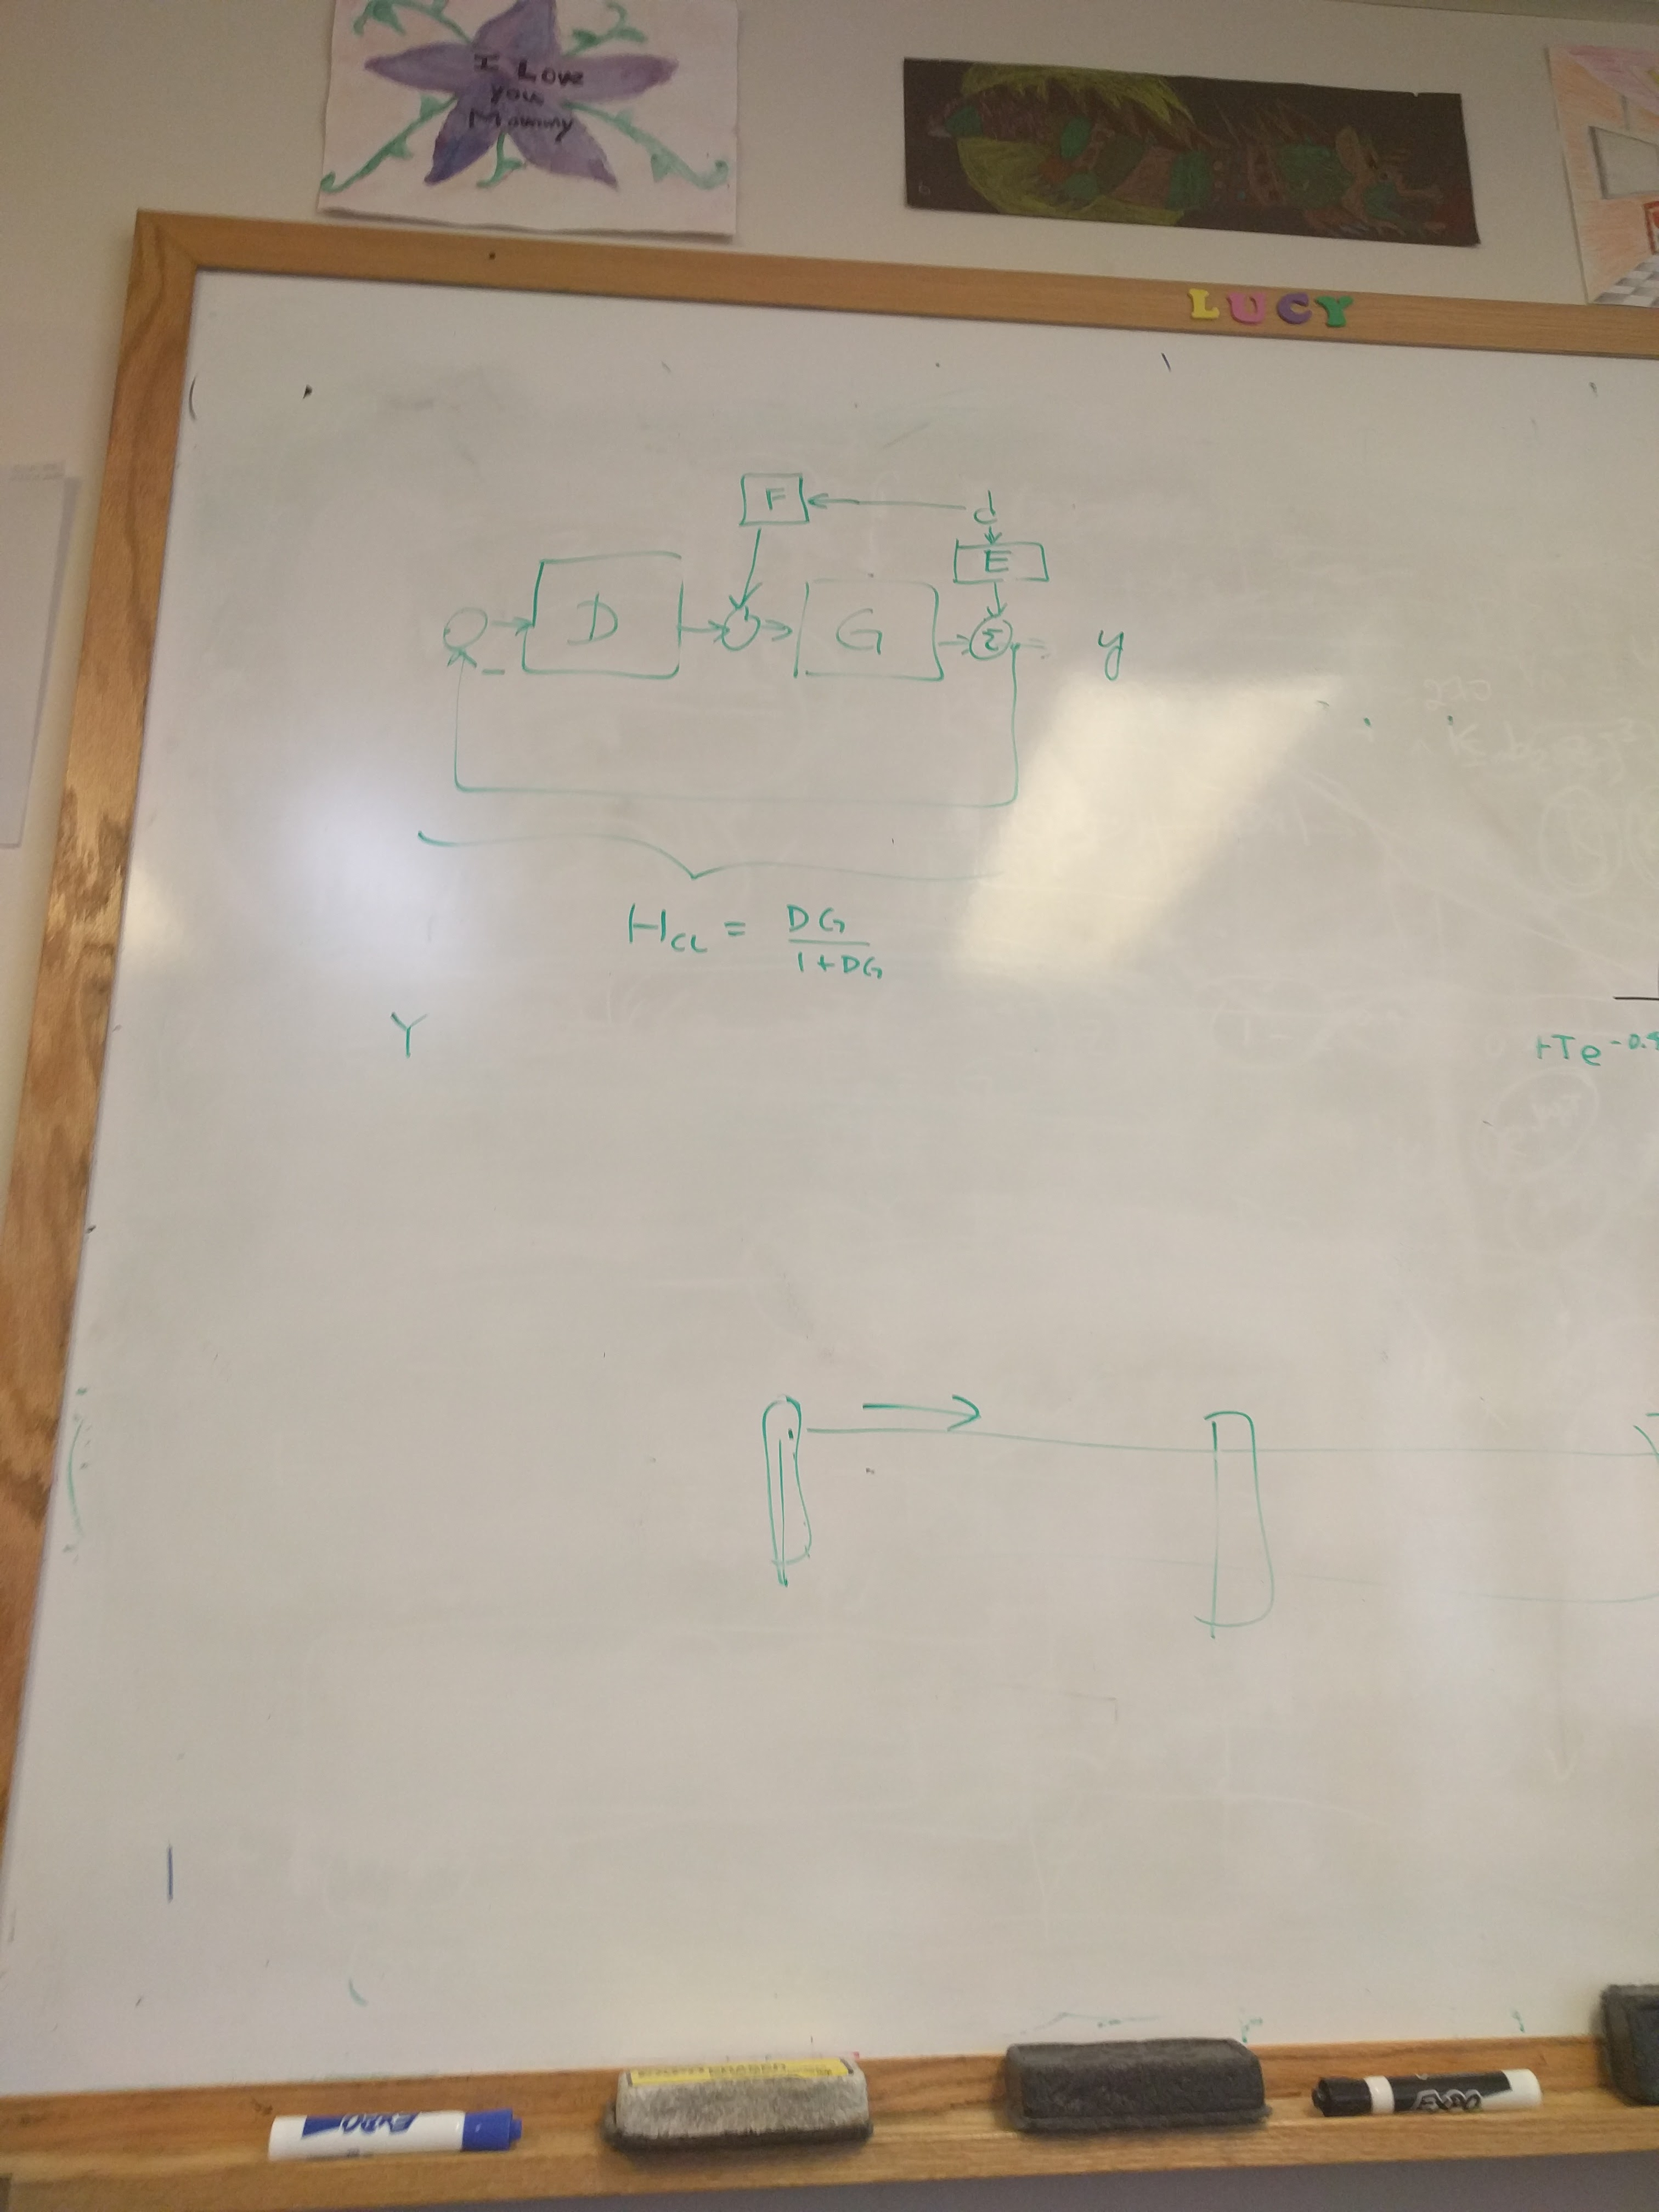
\includegraphics[width=0.8\textwidth]{pic3.jpg}
\end{figure}
\end{document}
